\lecture{11}{3 aprile 2024}
\section{Interferenza e battimenti}

Quando si parla di interferenza e di battimenti si utilizza la sovrapposizione di onde e quindi la linearità dell'equazione di D'Alembert. Utilizziamo onde armoniche perché tanto ogni onda periodica può essere scritta come sovrapposizione di onde armoniche e impulsi non periodici verranno comunque trattati tramite una trasformata di Fourier.

\subsection{Interferenza}
Per avere interferenze è necessario avere onde coerenti (per ora le consideriamo come onde sonore in un tubo), ovvero con la stessa identica pulsazione \(\omega \):
\begin{align}
	\xi _1 (x,t) &= A_1 \cos (kx - \omega t) & \xi _2 (x,t) &= A_2 \cos (kx - \omega t + \varphi_0 )
\end{align}
Passando nel piano complesso otteniamo che \(\xi _1 (x,t) = \Re [A_1 e^{i(kx- \omega t)}]\) e \(\xi _2 (x,t) = \Re [A_2 e^{i(kx- \omega t + \varphi _0)}]\). L'onda che si propaga è \(\xi (x,t)= \xi _1(x,t) + \xi _2 (x,t)\).
\begin{figure}[H]
	\centering
	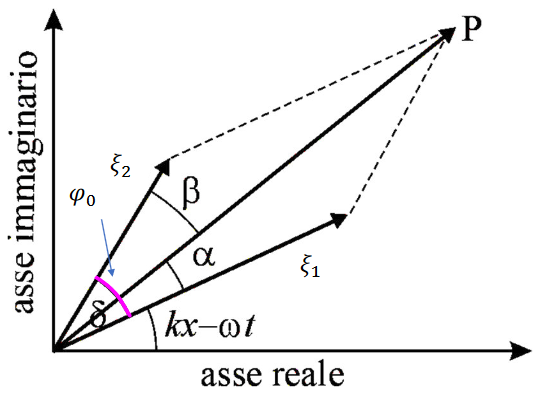
\includegraphics[width=0.6\textwidth]{screenshots/2024-04-03-09-23-02.png}
\end{figure}
Il punto P rappresenta il vettore \(\xi (x,t)\). Riscriviamo la funzione che descrive la posizione del punto P:
\begin{gather}
	\widetilde{\xi } (x,t) = A_1 e^{i(kx - \omega t)} + A_2 e^{i(kx - \omega t + \varphi _0)} =\\
	(A_1 + A_2 e^{i \varphi _0}) e^{i(kx - \omega t)} = A e^{i \alpha } e^{i(kx - \omega t)}
\end{gather}
Dove
\begin{gather}
	A  = \sqrt{A_1^2 + A_2^2 + 2A_1 A_2 \cos \varphi _0 }\\ 
\end{gather}
A seconda del valore di \(\varphi _0\) si possono presentare diversi casi:
\begin{description}
	\item[Ampiezza massima] per \(\varphi _0 = 0 \rightsquigarrow A = \vert A_1 + A_2 \vert \), è detta \emph{interferenza costruttiva}.
	\item[Ampiezza minima] per \(\varphi _0 = \pi \rightsquigarrow A = \vert A_1 - A_2 \vert \), è detta \emph{interferenza distruttiva}. In particolare, se \(A_1 = A_2\) e \(\varphi _0 = \pi \), allora \(A = 0\), ossia non ci sono onde!
\end{description}
Il termine \(2 A_1 A_2 \cos \varphi _0\) è detto termine di interferenza.
\paragraph{Intensità}
Ricordando che \(I_1 = \quotient{1}{2} Z \omega ^{2} A_1 ^{2} \) e \(I_2 = \quotient{1}{2} Z \omega ^{2} A_2 ^{2} \),
\[
	I = \frac{1}{2} Z \omega ^{2} A^{2} = \frac{1}{2} Z \omega ^{2} (A_1 ^{2} + A_2 ^{2} + 2 A_1 A_2 \cos \varphi _0 ) = I_1 + I_2 + 2 \sqrt{I_1 I_2} \cos \varphi _0
\]
Se le due onde hanno la stessa intensità \(I_1 = I_2 = I_0 \), allora 
\[
	I = 2 I_0 + 2 I_0 \cos \varphi _0 = 4 I_0 \cos ^{2} \left( \frac{\varphi _0}{2} \right)
\]
Se le onde sono in fase (interferenza costruttiva), ottengo che l'intensità risultante è quattro volte l'intensità di partenza: \(\varphi _0 = 0\), \(I= 4 I_0\). Se le onde sono invece in contro-fase (interferenza distruttiva), l'intensità risultante è nulla: \(\varphi _0 = \pi \), \(I = 0\).
\begin{note}
	Si sommano le onde complesse, ma non le ampiezza nè le intensità!
\end{note}

\subsection{Battimenti}
Consideriamo in questo caso due onde sonore armoniche con la stessa ampiezza (per semplicità, non è necessario) e pulsazioni simili \(\omega _1 \thickapprox  \omega _2\). Non siamo nel caso dell'interferenza perché le due pulsazioni non sono identiche. Viaggiando nello stesso mezzo, avremo anche che \(k_1 = k_2\).
\begin{align}
	\xi _1 (x,t) &= A \cos (kx - \omega _1 t) & \xi _2 (x,t) &= A \cos (kx - \omega _2 t)
\end{align}
Pongo \(\varphi _1 = k_1 x - \omega_1 t\) e \(\varphi _2 = k_2 x - \omega _2 t\). Passiamo immediatamente nel campo complesso: \(\widetilde{\xi } (x,t) = A (e^{i \varphi _1} + e^{i \varphi _2}) \).
\begin{figure}[H]
	\centering
	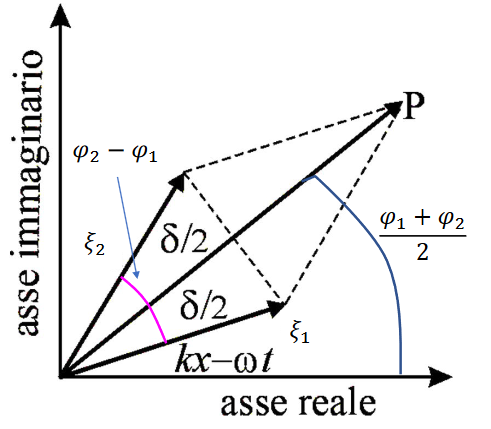
\includegraphics[width=0.6\textwidth]{screenshots/2024-04-03-09-44-52.png}
\end{figure}
Dalla figura si intuisce che \(A_{tot} = 2A \cos \left( \frac{\varphi _2 - \varphi _1}{2} \right) \) e che la fase \(\varphi _{tot} = \frac{\varphi _1 + \varphi _2}{2} \). Quindi, la funzione d'onda diventa:
\[
	\xi (x,t) = 2A \cos \left( \frac{\varphi _2 - \varphi _1}{2} \right) \cos \left( \frac{\varphi _1 + \varphi _2}{2} \right) 
\]
La somma non è un'onda armonica, perché entrambi i coseni dipendono dal tempo! Per comodità pongo \(\Delta k = \quotient{(k_2 - k_1)}{2} \), \(\Delta \omega = \quotient{(\omega _2 - \omega _1)}{2} \), \(k_0 = \quotient{(k_2 + k_1)}{1} \), \(\omega _0 = \quotient{(\omega _2 + \omega _1 )}{2} \), da cui:
\[
	\xi (x,t) = 2A \cos (\Delta k x - \Delta \omega t) \cos (k_0 x - \omega _0 t)
\]
Resta un'onda progressiva perché è un modo un po' più complicato di scrivere una dipendenza da \(x-vt\). I due coseni hanno periodi di oscillazione diversi: \(\tau = \quotient{2\pi}{\Delta \omega } \), \(T_0 = \quotient{2 \pi }{\omega _0} \), ma \(\omega _0 \gg \Delta \omega \), quindi \(\tau \gg T_0\).
I due termini hanno dei nomi precisi:
\begin{description}
	\item[Onda portante] \(\cos (k_0 x - \omega _0 t)\), velocemente variabile.
	\item[Onda modulante] \(2A \cos (\Delta k x - \Delta \omega t)\), lentamente variabile.
\end{description}
\(\omega _b = \omega _2 - \omega _1,\ \nu _b = \nu _2 - \nu _1\) sono detti pulsazione e frequenza di battimento rispettivamente. \(\omega _b = 2 \Delta \omega \) perché vi sono due massimi del battimento in un periodo di oscillazione dell'onda modulante. Il segno non conta perché tanto c'è la portante che fa oscillare velocemente fra \(-A_{mod} \) e \(+A_{mod} \).
Ma cosa sta succedendo?
\begin{figure}[H]
	\centering
	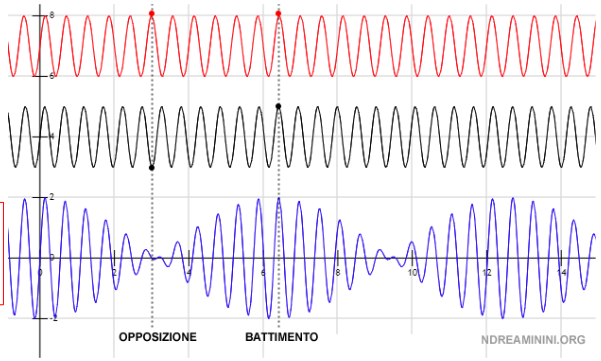
\includegraphics[width=0.6\textwidth]{screenshots/2024-04-03-09-55-54.png}
	\caption{Le onde rossa e nera sono le onde di partenza, l'onda blu è la somma delle due. Questo si può vedere molto bene usando un programma come Audacity.}
\end{figure}
Le fasi si muovono con velocità di fase \(v_f = \quotient{\omega _0}{k_0} \), mentre i massimi dell'inviluppo si muovono con velocità di gruppo \(v_g = \quotient{\Delta \omega }{\Delta k} \). Nei mezzi non dispersivi si ha che \(\omega (k) = vk\), quindi \(v_g = \frac{\mathrm{d} \omega }{\mathrm{d} k} = v = v_f \). Al contrario, nei mezzi dispersivi \(\omega (k) = k v(k)\), quindi \(v_g = \frac{\mathrm{d} \omega }{\mathrm{d} k} = v(k) + k \frac{\mathrm{d} v}{\mathrm{d} k}(k) \neq v_f \).
Sperimentalmente si verifica spesso \(v_g < v_f\), questo fenomeno è detto "dispersione normale". Nella trasmissione di segnali l'informazione viaggia con una velocità pari a \(v_g\), ovvero la velocità della modulazione e non della portante.
\begin{note}
	Non abbiamo utilizzato alcuna proprietà specifica delle onde sonore, questi fenomeni avvengono con ogni tipo di onda!
\end{note}

\section{Effetto Doppler}
L'effetto Doppler (classico) consiste nel cambiamento della frequenza dei suoni percepiti quando vi è moto relativo tra la sorgente e chi riceve le onde sonore. Un esempio è la sirena delle ambulanze. Chiameremo S la sorgente e R il ricevitore. I moti sono sempre valutati rispetto al sistema di riferimento in cui il mezzo è a riposo. Valutiamo i seguenti quattro casi:
\begin{enumerate}
	\item S e R fermi rispetto al mezzo.
	\item S in moto rispetto al mezzo, R fermo.
	\item R in moto, S fermo.
	\item Sia S che R in moto rispetto al mezzo.
\end{enumerate}
Immaginiamo che la sorgente invii un segnale semplice con una periodicità \(T_p\). Allora i suoni saranno emessi ai tempi \(t_{1s} = 0,\ t_{2s} = T_p,\ t_{3s} = 2T_p\).
\paragraph{Caso 1: S e R fermi}
\begin{figure}[H]
	\centering
	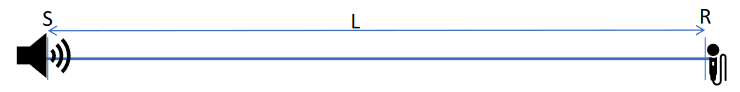
\includegraphics[width=0.7\textwidth]{screenshots/2024-04-03-10-33-12.png}
\end{figure}
Se \(v_m\) è la velocità delle onde nel mezzo e \(L\) è la distanza fra S e R, allora i tempi di arrivo saranno:
\begin{figure}[H]
	\centering
	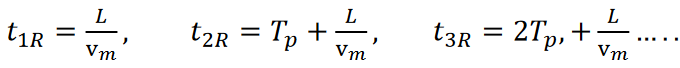
\includegraphics[width=0.7\textwidth]{screenshots/2024-04-03-10-34-50.png}
\end{figure}
Quindi la differenza di tempo d'arrivo fra due segnali è sempre \(T_p\), il che rende la frequenza sentita dal ricevitore identica alla frequenza emessa dalla sorgente.

\paragraph{Caso 2: S in moto, R fermo} Consideriamo la sorgente in moto con velocità \(v_s\) in avvicinamento al ricevitore.
\begin{figure}[H]
	\centering
	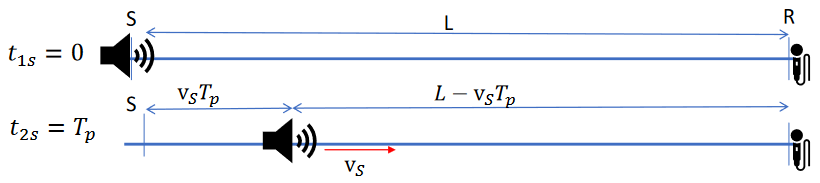
\includegraphics[width=0.7\textwidth]{screenshots/2024-04-03-10-36-23.png}
\end{figure}
Il tempo di ricezione del primo segnale è \(t_{1R} = \quotient{L}{v_m} \), mentre il tempo di ricezione del secondo segnale è
\begin{figure}[H]
	\centering
	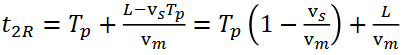
\includegraphics[width=0.4\textwidth]{screenshots/2024-04-03-10-38-48.png}
\end{figure}
Quindi l'intervallo dei segnali al ricevitore è
\begin{figure}[H]
	\centering
	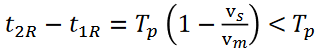
\includegraphics[width=0.4\textwidth]{screenshots/2024-04-03-10-39-19.png}
\end{figure}
La frequenza percepita dal ricevitore aumenta!
\[
	f_R = \frac{1}{T_p \left( 1- \frac{v_s}{v_m} \right) } = \frac{f_S}{1- \frac{v_s}{v_m}} > f_S
\]
Se vogliamo studiare il caso in cui la sorgente si allontana dal ricevitore, è sufficiente cambiare segno alla velocità \(v_s\). Si ottiene che
\[
	f_R = \frac{1}{T_p \left( 1+ \frac{v_s}{v_m} \right)  = \frac{f_s}{1 + \frac{v_s}{v_m}}} < f_S
\]

\paragraph{Caso 3: S ferma, R in moto} Il ricevitore è in moto a velocità \(v_R\) in avvicinamento alla sorgente.
\begin{figure}[H]
	\centering
	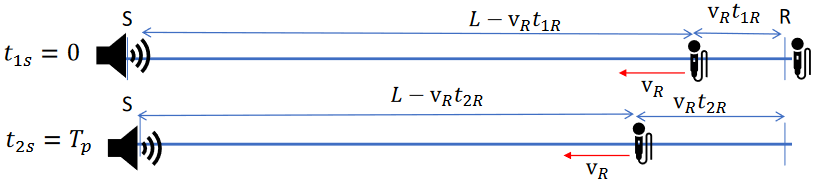
\includegraphics[width=0.7\textwidth]{screenshots/2024-04-03-10-44-02.png}
\end{figure}
Il primo segnale è emesso quando R dista \(L\) da S. Nel tempo di propagazione il ricevitore si è spostato di uno spazio pari a \(v_R t_{1R} \), quindi il segnale ha percorso uno spazio pari a \(L- v_R t_{1R} \). Si ottiene che
\[
	t_{1R} = \frac{L- v_R t_{1R} }{v_m} \rightsquigarrow t_{1R} = \frac{L}{v_m} \frac{1}{1+ \frac{v_R}{v_m}}
\]
Con un ragionamento analogo si ottiene che 
\[
	t_{nR}  = n T_p + \frac{L-v_R t_{2R} }{v_m} \rightsquigarrow t_{nR} = \frac{L}{v_m} \frac{1}{1 + \quotient{v_R}{v_m}} + \frac{n T_p}{1+ \quotient{v_R}{v_m} }
\]
Quindi l'intervallo fra i segnali ricevuti è
\begin{figure}[H]
	\centering
	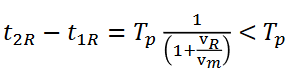
\includegraphics[width=0.4\textwidth]{screenshots/2024-04-03-10-49-27.png}
\end{figure}
Che ci permette di calcolare la frequenza percepita dal ricevitore:
\begin{figure}[H]
	\centering
	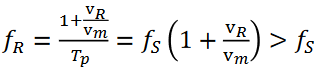
\includegraphics[width=0.4\textwidth]{screenshots/2024-04-03-10-49-54.png}
\end{figure}
Come nel caso 2, si può cambiare il segno della velocità \(v_R\) per studiare il caso in allontanamento:
\begin{figure}[H]
	\centering
	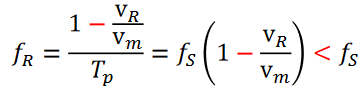
\includegraphics[width=0.4\textwidth]{screenshots/2024-04-03-10-50-52.png}
\end{figure}

\paragraph{Caso 4: S ed R in moto} Qui andiamo di ragionamento. Consideriamo il caso in cui S ed R sono entrambe in avvicinamento (per semplicità). Se la sorgente è in moto, le onde nel mezzo hanno una frequenza 
\[
	f_m = \frac{f_s}{1 - \quotient{v_S}{v_m} }
\]
come nel secondo caso, perché avevamo studiato un osservatore fermo, ossia solidale con il mezzo. Poiché il ricevitore è in moto le onde vengono ricevuta con un'altra frequenza:
\[
	f_R = f_m \left( 1+ \frac{v_R}{v_m} \right) = f_S \frac{1+ \frac{v_R}{v_m}}{1- \frac{v_S}{v_m}}
\]
Con ragionamenti simili a prima si ottiene la frequenza percepita dal ricevitore con altre combinazioni di velocità relative al mezzo.
\begin{note}
	Quanto fatto vale per qualunque onda meccanica con velocità dirette lungo la congiungente fra sorgente e ricevitore.
\end{note}